\documentclass{beamer}
%\usetheme{Ilmenau}
%\usecolortheme{beaver}

\usepackage[slovak,american]{babel}
\usepackage[utf8]{inputenc}
\usepackage{graphicx}
\usepackage{adjustbox}
 \usepackage{xcolor}
 
 \newsavebox\MBox
\newcommand\Cline[2][red]{{\sbox\MBox{$#2$}%
  \rlap{\usebox\MBox}\color{#1}\rule[-2.2\dp\MBox]{\wd\MBox}{1pt}}}

%\usefonttheme{serif}

\definecolor{UKOrange}{HTML}{ef9424} %
\definecolor{UKBrown}{HTML}{a96d5e} %
\definecolor{UKLight}{HTML}{d8b6ab} %
\definecolor{UKDark}{HTML}{7a4f44}
\definecolor{UKDarker}{HTML}{4d312b} 
\definecolor{UKDarkest}{HTML}{2e1e1a}
\definecolor{UKRed}{HTML}{bf1f1c}

\setbeamertemplate{footline}[frame number]{}
\setbeamertemplate{navigation symbols}{}

%\usecolortheme{beaver}
\setbeamertemplate{itemize item}[square]
\setbeamercolor{itemize item}{fg = UKBrown}
\setbeamercolor{itemize subitem}{fg = UKLight}
\setbeamercolor{enumerate item}{fg = UKDark}

\setbeamercolor{footnote}{fg=UKLight}
\setbeamercolor{footnote mark}{fg=UKLight}
\setbeamerfont{footnote}{size=\tiny}
\renewcommand\footnoterule{}

\usetheme{default}
\beamertemplatenavigationsymbolsempty
\setbeamercolor{title}{fg=white, bg=UKBrown}
\setbeamercolor{frametitle}{fg=white, bg=UKBrown}
\setbeamercolor{block title}{bg=UKBrown, fg= white}
\setbeamercolor{block body}{bg =UKLight, fg = UKDarkest}

\useoutertheme[subsection=false]{miniframes}
\AtBeginSection[]{\subsection{}}

\setbeamercolor{below lower separation line head}{bg=UKDark}
\addtobeamertemplate{headline}{}{%
  \begin{beamercolorbox}[colsep=0.5pt]{below lower separation line head}
  \end{beamercolorbox}
}
%\setbeamercolor*{mini frame}{fg=white,bg=UKRosy}
\setbeamercolor{section in head/foot}{fg=UKLight, bg=UKDark}

%\setbeamertemplate{itemize/enumerate body begin}{\normalsize}
%\setbeamertemplate{itemize/enumerate subbody begin}{\normalsize}




%\newcommand{\codeblock}[2]{ \begin{block}{#1} \begin{verbatim}#2\end{verbatim}\end{block}}

%\defbeamertemplate*{title page}{customized}[1][]
%{
%  \begin{centering}
%    \begin{beamercolorbox}[sep=8pt,center]{title}
%      \usebeamerfont{title}\inserttitle
%    \end{beamercolorbox}
%  \end{centering}
%  \bigskip
%
%\begin{columns}[onlytextwidth,T]
%
%
%  \column{27mm}
%  \includegraphics[width=27mm]{images/logoFMFI.png}
%  
%  \column{\dimexpr\linewidth-54mm-6mm}
%  \centering
%  \vspace{5mm}  
%  \usebeamerfont{author}\insertauthor\par
%  \vspace{5mm}
%  \usebeamerfont{institute}\insertinstitute\par
%
%  \column{27mm}
%  \includegraphics[width=27mm]{images/logoUK.png}  
%\end{columns}
%\centering
%\vspace{7mm}
%  \usebeamerfont{date}\insertdate\par
%}


\title[PCA a LDA]{Patter Recognition - 6th lab \\ Linear Classifier and SVM}
\author[Viktor Kocur]{Viktor Kocur \\{\small viktor.kocur@fmph.uniba.sk}}
\institute{DAI FMFI UK}
\date{30.3.2020}
%\titlegraphic{\includegraphics[width=2.7cm]{images/logoFMFI.png}\hspace*{1cm}~%
%   \includegraphics[width=2.7cm]{images/logoUK.png}
%}


\begin{document}
\selectlanguage{american}

\begin{frame}[plain]
  \titlepage  
\end{frame}

\section{Linear classifier}

\begin{frame}
\frametitle{Linear classifier}
\begin{block}{Basics}
The core principle of a linear classifier is a linear function $f : \mathbb{R}^n \mapsto \mathbb{R}, f(\vec{x}) = \vec{w}^T \vec{x} + b$, where $\vec{x}$ is the feature vector, $\vec{w}$ is the weight vector a $b$ is the bias term.
\end{block}

\begin{block}{Classification}
If we have two classes $\omega_1$ a $\omega_2$, then we add the feature vector $\vec{x}$ to the class $\omega_1$ if $f(\vec{x}) \ge 0$, and to class $\omega_2$ if $f(\vec{x}) < 0$.
\end{block}
\end{frame}



\begin{frame}
\frametitle{Linear classifier}
\begin{block}{Geometric interpretation}
The function $f$ divides the feature space into two areas divided by a hyperplane. Points where $f(\vec{x}) = 0$ lie exactly on this hyperplane.
\end{block}

\begin{block}{Training}
We want to find the parameters of our classifier so that the hyperplane separates the training set the best.
\end{block}
\end{frame}


\begin{frame}
\frametitle{Linear classifier}
\center
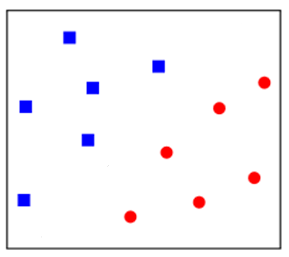
\includegraphics[width=0.8\textwidth]{lc1.png}
\end{frame}


\begin{frame}
\frametitle{Linear classifier}
\center
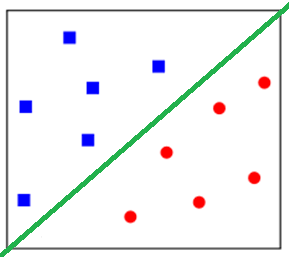
\includegraphics[width=0.8\textwidth]{lc2.png}
\end{frame}

\begin{frame}
\frametitle{Training}
\begin{block}{Training}
To train the classifier we will need the so-called training data. E.g. pairs of feature vectors $\vec{x}$ with labels $y \in \{0,1\}$ determined by the correct class. Our goal is for the classifier to work well on the training data.
\end{block}

\begin{block}{Regularization}
Sometimes we want a classifier which is not the best one possible on the training data. Instead we want one that can generalize well. This kind of approach is called regularization.
\end{block}
\end{frame}

\begin{frame}
\frametitle{Cost function - I}
\begin{block}{Cost function}
We obtain a good classifier by creating a cost function $C : \mathbb{R}^{n+1} \mapsto \mathbb{R}, C(b, \vec{w})$, which has a global minimum for parameters which separate the classes the best. Training is then an optimization task.
\end{block}
\end{frame}

\begin{frame}
\frametitle{Cost function - II}
\begin{block}{Simplification}
Since the bias term $b$ complicates things a bit we will use new notation $\vec{\theta} = (b, \vec{w})$ and $\vec{X} = (1, \vec{x})$. Such a change enables us to use the expression: $f(\vec{X}) = \vec{\theta}^T \vec{X}$.
\end{block}

\begin{block}{Sigmoid}
We will use the sigmoid function: $\sigma(z) = \frac{1}{1+e^{-z}}$.
\end{block}

\begin{block}{Sigmoid - derivative}
$\sigma(z)' = \sigma(z) (1 - \sigma(z))$.
\end{block}
\end{frame}


\begin{frame}
\frametitle{Sigmoid}
\center
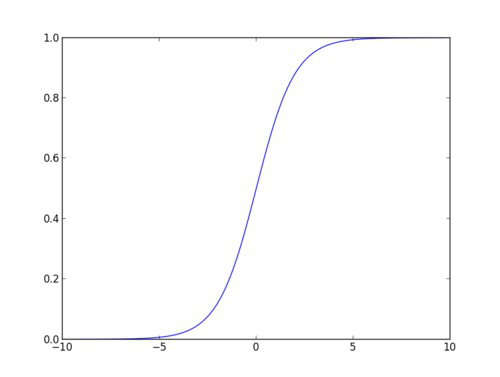
\includegraphics[width=0.8\textwidth]{sigmoid.png}
\end{frame}



\begin{frame}
\frametitle{Cost function - III}
\begin{block}{Simplification}
Let us consider a function: $h_{\theta} = \sigma(f(\vec{x}))$.
\end{block}

\begin{block}{Cost function - binary crossentropy}
\begin{equation*}
J(\vec{\theta}) = \frac{1}{m} \sum_{i=1}^m \left( -y^{(i)} log(h_{\theta}(\vec{x}^{(i)})) - (1 - y^{(i)}) log(1 - h_{\theta} (\vec{x}^{(i)})) \right)
\end{equation*}
\end{block}

\begin{block}{Cost function - derivative}
\begin{equation*}
\frac{\partial J}{\partial \theta_j} = \frac{1}{m} \sum_{i=1}^m \left( h_{\theta}(\vec{x}^{(i)}) - y^{(i)} \right) x_j^{(i)}
\end{equation*}
\end{block}
\end{frame}


\begin{frame}
\frametitle{Optimizataion}
\begin{block}{Gradient descent}
$\theta_i := \theta_i - \eta \frac{\partial J}{\partial \theta_i}$
\end{block}

\begin{block}{Optimization in reality}
Usually the optimization is performed using a more sophisticated algorithm such as SGD, or methods based on the Hess matrix.
\end{block}

\begin{block}{Optimization in Matlab}
x = fminunc(fun,x0) - finds the optimal parameters where the function fun is minimal. Since this function uses iterative methods it is necessary to add initial value x0.
\end{block}
\end{frame}

\begin{frame}
\frametitle{Optimization}
\begin{block}{Exercise}
Check the LinearClassifier.m script.
\end{block}

\begin{block}{Exercise}
Finish the function costFunction using the cost function we introduced few slides back.
\end{block}
\end{frame}



\begin{frame}
\frametitle{Linear classifier - Matlab}
\begin{block}{Regularization}
We add a regularization term to the cost function: $C_R(\vec{\theta}) = C(\vec{\theta}) + R(\vec{\theta})$. For example $R(\vec{\theta}) = \sum_{i=2}^n \theta_i^2$, or $\sum_{i=2}^n |\theta_i |$
\end{block}


\begin{block}{fitclinear}
Mdl = fitclinear(x,y) - returns a classification model Mdl for feature vectors which are in rows of matrix x and correct classes in y. This function can perform SVM and logistical regression. Check out help. Regularization is used by default.
\end{block}

\begin{block}{Mdl.predict}
Mdl.predict(x) - returns the class for given feature vector
\end{block}
\end{frame}


\begin{frame}
\frametitle{Linear classifier - Matlab}
\begin{block}{Mdl.Beta, Mdl.Bias}
Mdl.Beta - returns our weight vector $\vec{w}$. Mdl.Bias - returns the bias term $b$.
\end{block}


\begin{block}{Exercise}
Into the image (gscatter) with data from ex2data1.txt add the line which separates the data for fitcliniear classifier. You can use plot or refline commands. Note for refline we use:
$$\beta_1 \cdot x_1 + \beta_2 \cdot x_2 + bias = 0 \iff  x_2 = m \cdot x_1 + b $$
$$x_2 = -\frac{\beta_1}{\beta_2} \cdot x_1 - \frac{bias}{\beta_2}$$
$$ m = -\frac{\beta_1}{\beta_2}, b = - \frac{bias}{\beta_2}$$
\end{block}
\end{frame}

\section{SVM}

\begin{frame}
\frametitle{Idea of SVM}
\center
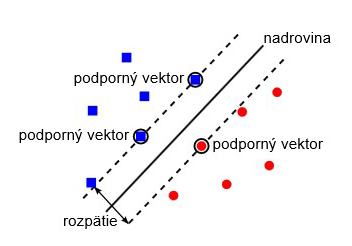
\includegraphics[width=0.8\textwidth]{svm.png}
\end{frame}

\begin{frame}
\frametitle{SVM}
\begin{block}{Basics}
SVM finds support vectors and attempts to find paramaters so that the gap between the classes is the widest. This is achieved by trying to find parametrization so that $\vec{w}^T \vec{x} + b = \pm 1$ for the support vectors.
\end{block}

\begin{block}{Kernels}
Data is usually not linearly separable. Therefore it is necessary to transform the feature space using so-called kernels. Kernels are functions $\phi : \mathbb{R}^n \mapsto \mathbb{R}^{m}$, for which a function $k$ exists so that: $k(x_i, x_j) = \phi(x_i) \phi(x_j).$ SVM then finds a linear classifier in the new space  $\mathbb{R}^m$.
\end{block}
\end{frame}


\begin{frame}
\frametitle{SVM}
\begin{block}{fitcsvm}
SVMMdl = fitcsvm(X,y) - returns an SVM model on features X and classes y.
\end{block}

\begin{block}{fitcsvm}
SVMMdl = fitcsvm(X,y, 'KernelFunction',nazov, 'KernelScale', 'auto') - returns an SVM with kernel trick. Note: do not forget the scale.
\end{block}
\end{frame}


\begin{frame}
\frametitle{SVM - Úloha}
\begin{block}{showSVM}
showSVM(SVMMdl, X, y) - displays the SVM model for 2D data X,y (this is an m-file in the zip)
\end{block}

\begin{block}{Exercise}
Display an SVM with various kernels. Check out what happens when you do not set the KernelScale.
\end{block}
\end{frame}

\end{document}